\section{Theorie}
\label{sec:Theorie}

\subsection{Tomographie}

Tomographie bezeichnet ein Verfahren bei den schichtweise Aufnahmen von einem Objekt genommen werden, um so dessen innere Zusammensetzung darzustellen.
In diesen Versuch wird mithilfe von der Absorption von Gammastrahlung die Zusammensetzung eines Würfels aus 3x3x3 einzelnen Würfeln bestimmt.
Dazu wird erst die Interaktion von Gammastrahlung mit Materie beschrieben.

\subsection{Interaktion Gamma-Strahlung mit Materie}

Beim Durchlauf von Gamma-Strahlung durch feste Materie kann das $\gamma$-Quant auf 3 verschiedene Arten wechselwirken.

Bei den photoelektrischen Effekt wechselwirkt das $\gamma$-Quant mit den Hüllenelektronen und löst diese aus ihrer Position in der Schale. Dabei wird die gesamte Energie des Photons an das Elektron übertragen.
Die Wahrscheinlichkeit das ein Teilchen absorbiert wird mit der  Wirkungsquerschnitt $\tau$ ausgedrückt, welche von der Atomzahl Z des Materials und der Energie des $\gamma$-Quants $E_\gamma$ abhängt. 
\begin{equation*}
    \tau \propto Z^n / E_\gamma^m \,
\end{equation*}
n und m sind dabei wiederum abhängig von der Teilchen-Energie und in einen Bereich zwischen 3 und 5.
Der Absorptionskoeffizient, welcher ein Maß für die absorbierte Strahlung ist, ist somit:
\begin{equation}
    \mu_{PE} = \tau  \rho  N_A/A \,.
\end{equation}
Dabei ist \rho die Dichte des Materials, $N_A$ die Avogadro Konstante und A die Massenzahl.

Die Comptonstreuung ist die inelastische Streuung eines Photons mit einem Elektron. Die Energie des Photons wird dabei nur teilweise an das Elektron abgegeben.
Der Wirkungsquerschnitt $\sigma$ dieses Vorganges hängt dabei, ähnlich wie der photoelektrische Effekt,  mit der Atomzahl Z des Materials und der Energie des Photons zusammen 
\begin{equation*}
    \sigma \propto f(E_\gamma) \propto 1/E_\gamma\,.
\end{equation*}
Mit der Annahme, dass das Verhältnis A/Z ist für einen Großteil des Periodensystems konstant ist, lässt sich der Absorptionskoeffizient für Comptonstreuung als 
\begin{equation}
    \mu_{CS} = \text{constant} \cdot \sigma \cdot f(E_\gamma)
\end{equation}
angeben. 

Bei der Paar-Produktion wechselwirkt das $\gamma$-Quant mit dem Coulomb-Feld des Atomkerns. Dort zerfällt es  in ein Elektron-Positron-Paar. Damit muss das Photon mindestens die Energie von 2 Elektronen Massen haben um diese erzeugen zu können.
Der Wirkungsquerschnitt der Paar-Produktion ist nicht trivial zu bestimmen, hängt dabei aber von der Atomzahl Z und Strahlungsenergie $E_\gamma$ ab.
\begin{equation*}
    \kappa \propto Z^2f(E_\gamma, Z) 
\end{equation*}
Der Absorptionskoeffizient lässt sich analog zu den des photoelektrischen Effektes berechnet.

Die gesamte Absorption ist die Überlagerung aller Effekte. Damit ist der Absorbtionskoeffizient insgesamt
\begin{align}
    \mu_T &= \mu_{PE} + \mu_{CS} + \mu_{PP} + \mu_{RS} \\
        &  =(\rho  N_A/A) (\tau + \sigma + \kappa + \sigma_{RS}) \,.
\end{align}
Meist wird jedoch das Verhältnis zwischen Absorptionskoeffizient und Dichte des Materials angegeben:
\begin{equation}
    \mu_t / \rho = (N_A/A)(\tau + \sigma + \kappa + \sigma_{RS}) \,.
\end{equation}

\begin{figure}
    \centering
    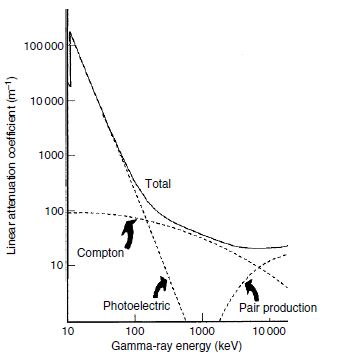
\includegraphics[width=0.9\textwidth]{content/attenuation.jpg}
    \caption{Absorptionskoeffizienten für die einzelnen Wechselwirkungsporzesse, sowie der Absorptionskoeffizient der gesamten Absorption an Beispiel von Germanium. \cite{Gilmore}}
    \label{fig:plot}
\end{figure}

\subsection{Messelektronik}

Die radioaktive Strahlung wird in diesen Versuch mittels eines Szintillationsdetektor gemessen. Ein Szintillator ist ein Material, welches einfallende Strahlung in Photonen umwandelt.
In einen kristallinen Szintillator werden durch Dotierung Fremdatome in die Kristallstruktur eingebracht. 
Einfallendende Gammastrahlung kann Elektronen aus dem Valenzband in das Leitungsband heben. Dabei entstehen Elektronen-Loch-Paare, die sich frei im Kristall bewegen können. Diese wechselwirken mit den Fremdatomen, welche dabei angeregt werden. Unter Abgabe eines Photons fallen sie nach kurzer Zeit wieder in den Grundzustand zurück.

In einen nachgeschalteten Photomultiplier werden diese Photonen in Elektronen umgewandelt und verstärkt. 
Ein Photomultiplier besteht aus einer Photokathode, aus der  mittels den photoelektrischen Effekt einfallenden Photonen Elektronen freisetzen. Diese werden mittels einer angelegten Spannung Richtung der Dynoden beschleunigt. Beim Aufprall der beschleunigten Elektronen werden weitere Elektronen freigesetzt. 
An Ende des Photomulipliers werden die so gewonnenen Elektronen an einer Anode gesammelt und es entsteht eine messbare elektrische Puls.

Mittels eines Multichannelanalyser wird dieser Puls ausgewertet.
Der einkommende Puls ladet dabei einen Kondensator. Dieser wird danach sofort wieder entladen und die dafür benötigte Zeit, welche proportional zu Pulshöhe ist, wird aufgenommen. Diese Ereignisse werden dann in zu den aufgenommenen Zeiten zugeordneten Registern aufaddiert.


\subsection{Berechnung der Absorptionskoeffizienten}

Die Intensität von Gammastrahlung nach dem Durchgang durch Materie lässt sich mit der Formel
\begin{equation}
    I = I_0 \exp(-\sum_i \mu_i d_i)
\end{equation}
berechnen.
Dabei ist $I_0$ die Eingangsintensität des Strahls, $\mu_i$ der Absorptionskoeffizient und $d_i$ die Schichtdicke der i-ten Schicht.
Dies lässt sich umstellen nach
\begin{equation}
    \ln(\frac{I_0}{I}) = \sum_i \mu_i d_i \,.
\end{equation}
Mit der Matrixdarstellung ergibt sich dann für mehrere Messungen die Formel
\begin{equation}
    \label{eqn:matrixA}
    \vec{I} = A \vec{\mu} \,.
\end{equation}
Die Spalten von A stellen dabei den i-ten Block dar und die Zeilen jeweils die j-te Messung. Die einzelnen Einträge sind dabei die Strecke die der Strahl bei der jeweiligen Messung durch einen gegebenen Block genommen hat. Damit geben sie auch an, welchen Weg der Strahl durch den Block genommen hat.
Damit das Gleichungssystem lösbar ist, muss die Matrix mindestens denselben Rang haben wie die Dimension von $\vec{mu}$. 
In diesem Versuch werden mehr Messungen gemacht wodurch das Gleichungssystem überbestimmt wird. Mit der Methode der kleinsten Quadrate und unter der Berücksichtigung von Gleichung \ref{eqn:matrixA} lässt sich die Gleichung 
\begin{align}
    W A \cdot \vec{\mu} = W \vec{I}
\end{align}
herleiten. Dabei ist $W$ die Gewichtungsmatrix mit 
\begin{align}
    W = V[I] ^{-1}.
\end{align}

Dadurch ergibt sich für die Absorbtionskoeffizienten die Gleichung 
\begin{align}
    \label{eqn:mu}
    \vec{\mu} = (A^T W A)^{-1} (A^T W \vec{I})
\end{align}
mit den Unsicherheiten
\begin{align}
    V[\mu] = (A^T W A)^{-1}.
\end{align}
Die Varianzmatrix $V$ ist definiert als die Inverse der Gewichtungsmatrix, da die Unsicherheiten Poisson-verteilt sind. 